\section{Test Description and Success Criteria}
This test is located in \texttt{SimCode/dynamics/HingedRigidBodies/UnitTest/\newline
test\_hingedRigidBodyStateEffector.py}. In this integrated test there are two hinged rigid bodies connected to the spacecraft hub.  Depending on the scenario, there are different success criteria. These are outlined in the following subsections:
\subsection{Gravity and no damping scenario}
In this test the simulation is placed into orbit around Earth with point gravity and has no damping in the hinged rigid bodies. The following parameters are being tested. 
\begin{itemize}
	\item Conservation of orbital angular momentum
	\item Conservation of orbital energy
	\item Conservation of rotational angular momentum
	\item Conservation of rotational energy
	\item Achieving the expected final attitude
\end{itemize}

\subsection{No gravity and no damping scenario}
In this test, the spacecraft is placed in free space (no gravity) and has no damping in the hinged rigid bodies. The following parameters describe the success criteria.
\begin{itemize}
\item Conservation of orbital angular momentum
\item Conservation of orbital energy
\item Conservation of rotational angular momentum
\item Conservation of rotational energy
\item Achieving the expected final attitude (same final attitude as the Gravity with no damping scenario)
\item Achieving the expected final position
\item Conservation of velocity of center of mass
\end{itemize}

\subsection{No gravity with damping scenario}
In this test, the spacecraft is placed in free space (no gravity) and has damping in the hinged rigid bodies. The following parameters describe the success criteria.
\begin{itemize}
\item Conservation of orbital angular momentum
\item Conservation of orbital energy
\item Conservation of rotational angular momentum
\item Conservation of velocity of center of mass
\end{itemize}

\subsection{Steady State Deflection Verification Scenario}

The BOE calculation for the steady state deflection can be seen in Fig.~\ref{fig:BOEThetaSS}. The resulting steady state deflection does not have a closed form solution so a root solving function must be used to converge on the solution. A Newton-Raphson method was chosen and the success criteria for this test is whether Basilisk gives the same results as this BOE calculation within a certain tolerance. The spacecraft has a constant force applied through the whole simulation with the hinged rigid bodies initially undeflected and they have damping. The force is always applied through the center of mass of the spacecraft and results in no rotation of the spacecraft. 

\begin{figure}[htbp]
	\centerline{
		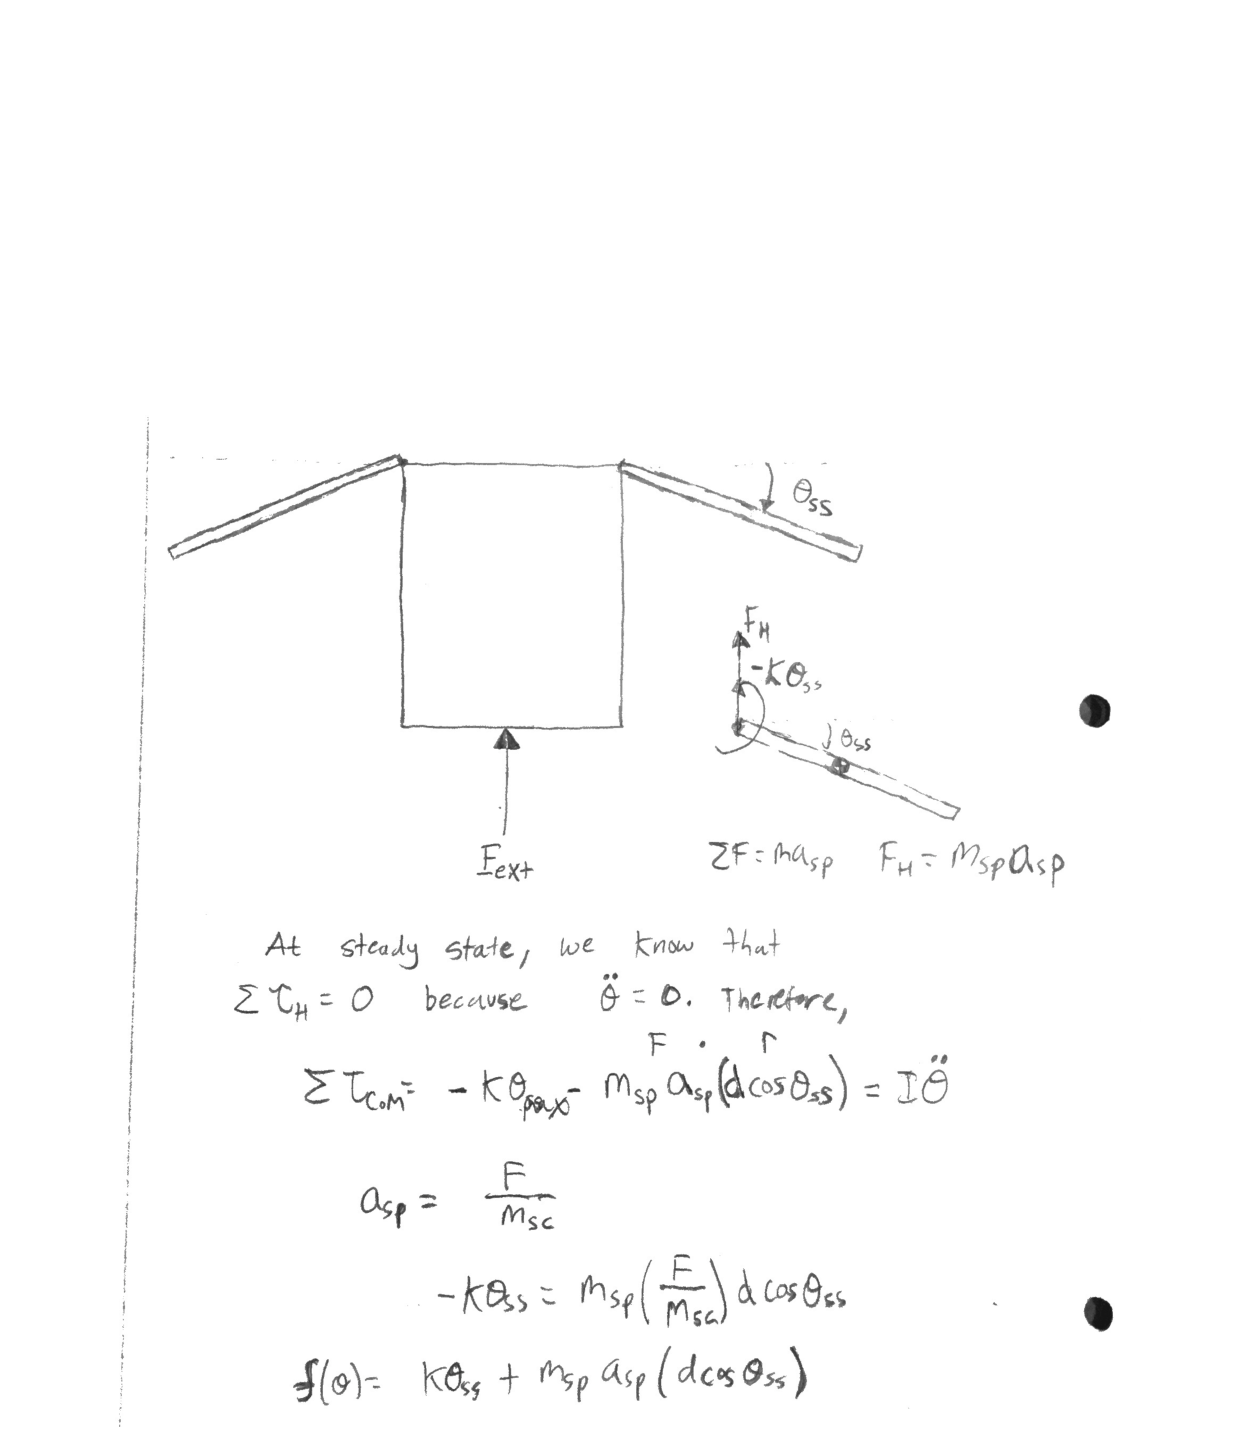
\includegraphics[width=0.8\textwidth]{Figures/BOEThetaSS}}
	\caption{Steady State Deflection BOE Calculation}
	\label{fig:BOEThetaSS}
\end{figure}

\subsection{Frequency and Amplitude Verification Scenario}

\subsubsection{Frequency Test Description}

The BOE calculation for the frequency of oscillation of flexing hinged rigid bodies when a constant force is being applied to the spacecraft is done by making simplifications to the flexing equation seen in the Model Description Section. The following assumptions are made to simplify the equations:

\begin{enumerate}
	\item The force is being directed through the center of mass of the spacecraft, along the $\hat{\bm b}_2$ direction
	\item The panels are initially undeflected and they are symmetric therefore the body will not rotate
	\item Rotation is no longer apart of the equations so the translation and solar panel equations are the only equations needed
	\item $\hat{\bm s}_{i,3}$ is assumed to be equal to $\hat{\bm h}_{i,3}$ in the equations of motion \label{item:4}
	\item No external torque is being applied directly to the hinged rigid bodies
	\item Non-linear terms are neglected \label{item:5}
\end{enumerate}
Using the third assumption from above, the rotational motion is taken out of the equations of motion:

\begin{equation}
m_{\text{sc}} \ddot{\bm r}_{B/N}+\sum_{i}^{N}m_{\text{sp}_i} d_i  \bm{\hat{s}}_{i,3}\ddot{\theta}_i = \bm F_{\textnormal{ext}} -\sum_{i}^{N}m_{\text{sp}_i}d_i\dot{\theta}_i^2 \bm{\hat{s}}_{i,1}
\label{eq:Rbddot6}
\end{equation}

\begin{equation}
m_{\text{sp}_i} d_i \hat{\bm s}_{i,3}^{T} \ddot{\bm r}_{B/N} 
+ \left( I_{s_{i,2}} + m_{\text{sp}_i} d_i^{2} \right) \ddot \theta_i 
= - k_i \theta_i - c_i \dot\theta_i + \hat{\bm s}_{i,2}^T \bm \tau_{\text{ext},H_i}  
\label{eq:solar_panel_final9}
\end{equation}
Next, assumptions \ref{item:4}-\ref{item:5} are applied:
\begin{equation}
m_{\text{sc}} \ddot{\bm r}_{B/N}+\sum_{i}^{N}m_{\text{sp}_i} d_i  \bm{\hat{h}}_{i,3}\ddot{\theta}_i = \bm F_{\textnormal{ext}}
\label{eq:Rbddot7}
\end{equation}

\begin{equation}
m_{\text{sp}_i} d_i \hat{\bm h}_{i,3}^{T} \ddot{\bm r}_{B/N} 
+ \left( I_{s_{i,2}} + m_{\text{sp}_i} d_i^{2} \right) \ddot \theta_i 
= - k_i \theta_i - c_i \dot\theta_i  
\label{eq:solar_panel_final10}
\end{equation}
Finally, knowing that the force is being directed along the $\hat{\bm b}_2$ axis and that the spacecraft will not rotate, the equations simplify to:
\begin{equation}
m_{\text{sc}} \ddot{y}_{B/N}+\sum_{i}^{N}m_{\text{sp}_i} d_i \ddot{\theta}_i = F_{y}
\label{eq:Rbddot9}
\end{equation}

\begin{equation}
m_{\text{sp}_i} d_i \ddot{y}_{B/N} 
+ \left( I_{s_{i,2}} + m_{\text{sp}_i} d_i^{2} \right) \ddot \theta_i 
= - k_i \theta_i - c_i \dot\theta_i  
\label{eq:solar_panel_final12}
\end{equation}
Converting these equations to state space:
\begin{multline}
\begin{bmatrix}
1 & 0 & 0 & 0 & 0 & 0\\
0 & m_{\text{sc}} & 0 & m_{\text{sp}_1} d_1 & 0 & m_{\text{sp}_2} d_2 \\
0 & 0 & 1 & 0 & 0 & 0\\
0 & m_{\text{sp}_1} d_1 & 0 &  I_{s_{1,2}} + m_{\text{sp}_1} d_1^{2} & 0 & 0 \\
0 & 0 & 0 & 0 & 1 & 0\\
0 & m_{\text{sp}_2} d_2 & 0 & 0 & 0 & I_{s_{2,2}} + m_{\text{sp}_2} d_2^{2} \\
\end{bmatrix}
\begin{bmatrix}
\dot{y}_{B/N} \\
\ddot{y}_{B/N} \\
\dot \theta_1 \\
\ddot \theta_1 \\
\dot \theta_2 \\
\ddot \theta_2 \\
\end{bmatrix}
\\
=\begin{bmatrix}
0 & 1 & 0 & 0 & 0 & 0\\
0 & 0 & 0 & 0 & 0 & 0\\
0 & 0 & 0 & 1 & 0 & 0\\
0 & 0 & -k_1 & -c_1 & 0 & 0\\
0 & 0 & 0 & 0 & 0 & 1\\
0 & 0 & 0 & 0 & -k_2 & -c_2\\
\end{bmatrix}
\begin{bmatrix}
{y}_{B/N} \\
\dot{y}_{B/N} \\
\theta_1 \\
\dot \theta_1 \\
\theta_2 \\
\dot \theta_2 \\
\end{bmatrix}
+ \begin{bmatrix}
0 \\
F_y \\
0 \\
0 \\
0 \\
0 \\
\end{bmatrix}
\label{eq:solar_panel_final13}
\end{multline}
Written in a more compact form:
\begin{equation}
[M] \dot{\bm X} = [A] \bm X + \bm F
\end{equation}
The equivalent dynamics matrix for this coupled system is:
\begin{equation}
[\tilde{A}] = [M][A]
\end{equation}

Finding the eigenvalues of $[\tilde{A}]$ will describe the coupled natural frequencies of the combined system. The integrated test for this scenario ensures that the analytical coupled frequency of oscillation matches the frequency obtained from the simulation. 

\subsubsection{Max Deflection While Force is Being Applied}

The next BOE calculation that is needed is to find the maximum deflection while the force is being applied and when the force is not being applied (with the assumption that there is no damping). When the force is being applied the following max deflection can be seen in the following equation:

\begin{equation}
\theta_{\textnormal{max}} = 2 \theta_{\textnormal{SS}}
\end{equation}
which uses the definition of $\theta_{\textnormal{SS}}$ from Fig.~\ref{fig:BOEThetaSS}. 

\subsubsection{Max Deflection While Force is Not Being Applied}

Finally, the maximum deflection when the force is not being applied uses energy techniques. Once the force is no longer being applied, energy is conserved and the velocity of the center of mass is constant. The energy when the force is turned off is represented in the following equation:

\begin{equation}
E_0 = \frac{1}{2} m_{\textnormal{hub}} \dot{y}_{B/N}^2 + 2\Big[\frac{1}{2} m_{\textnormal{sp}} \dot{\bm r}_{\textnormal{sp}} \cdot \dot{\bm r}_{\textnormal{sp}}  +  \frac{1}{2} I_{\textnormal{sp}} \dot{\theta}^2 + \frac{1}{2} k \theta^2\Big]
\end{equation}
Where $\dot{\bm r}_{\textnormal{sp}}$ is
\begin{equation}
\dot{\bm r}_{\textnormal{sp}} = \begin{bmatrix}
-d \dot{\theta} \sin (\theta)\\
\dot{y}_{B/N}  + d \dot{\theta} \cos (\theta)\\
\end{bmatrix}
\end{equation}
Next, the velocity of the center of mass of the system is defined in the following equation:
\begin{equation}
v_{\textnormal{CoM}} = \frac{1}{m_{\textnormal{tot}}}(m_{\textnormal{hub}} \dot{y}_{B/N} + 2 m_{\textnormal{sp}}\dot{ r}_{\textnormal{sp},y})
\end{equation}
This value can be computed from the values at the time the force is shut off and is a conserved quantity.

When the panels are deflected at max deflection, $\dot{\theta} = 0$. Leveraging this assumption the final energy is defined as follows:
\begin{equation}
E_F = \frac{1}{2} m_{\textnormal{tot}} v_{\textnormal{CoM}}^2 + 2\Big[\frac{1}{2} k \theta_{\textnormal{max}}^2\Big]
\end{equation}
Conservation of energy states
\begin{equation}
E_0 = \frac{1}{2} m_{\textnormal{tot}} v_{\textnormal{CoM}}^2 + k \theta_{\textnormal{max}}^2
\end{equation}
Therefore, $\theta_{\textnormal{max}}$ is found using the following equation:
\begin{equation}
\theta_{\textnormal{max}} = \sqrt{\frac{E_0 - \frac{1}{2} m_{\textnormal{tot}} v_{\textnormal{CoM}}^2}{k}}
\end{equation}

\subsection{Lagrangian vs Basilisk Scenario}

In this scenario the equations of motion for a planar simulation of a spacecraft hub and two hinged rigid bodies using Lagrangian mechanics was developed using Mathematica. The mathematica script can be seen in the support folder in the following file name: PlanarFlexibleDynamicsDerivation. This simulation is ran independently in the integrated test and the results are compared vs Basilisk results. A force and torque is applied for a certain amount of time, then turned off. Then another pulse of a force and torque is applied and turn off and the simulation runs for another few seconds.

\section{Test Parameters}

Since this is an integrated test, the inputs to the test are the physical parameters of the spacecraft along with the initial conditions of the states. These parameters are outlined in Tables~\ref{tab:hub}-~\ref{tab:initial}. Additionally, the error tolerances can be seen in Table~\ref{tab:errortol}.

\begin{table}[htbp]
	\caption{Spacecraft Hub Parameters}
	\label{tab:hub}
	\centering \fontsize{10}{10}\selectfont
	\begin{tabular}{| c | c | c | c |} % Column formatting, 
		\hline
		\textbf{Name}  & \textbf{Description}  & \textbf{Value} & \textbf{Units} \\
		\hline
		mHub  & mass & 750.0 & kg \\
		\hline
		IHubPntBc\_B & Inertia in $\cal{B}$ frame & $\begin{bmatrix}
		900.0 & 0.0 & 0.0\\
		0.0 & 600.0 & 0.0\\
		0.0 & 0.0 & 600.0
		\end{bmatrix}$ & kg-m$^2$ \\
		\hline
		r\_BcB\_B & CoM Location in $\cal{B}$ frame & $\begin{bmatrix}
		0.0 & 0.0 & 1.0 \end{bmatrix}^T$ & m \\
		\hline
	\end{tabular}
\end{table}

\begin{table}[htbp]
	\caption{Hinged Rigid Body 1 Parameters}
	\label{tab:panel1}
	\centering \fontsize{10}{10}\selectfont
	\begin{tabular}{| c | c | c | c |} % Column formatting, 
		\hline
		\textbf{Name}  & \textbf{Description}  & \textbf{Value} & \textbf{Units} \\
		\hline
		mass  & mass & 100.0 & kg \\
		\hline
		IPntS\_S & Inertia in $\cal{S}$ frame & $\begin{bmatrix}
		100.0 & 0.0 & 0.0\\
		0.0 & 50.0 & 0.0\\
		0.0 & 0.0 & 50.0
		\end{bmatrix}$ & kg-m$^2$ \\
		\hline
		d & CoM location & 1.5 & m \\
		\hline
		k & Spring Constant & 100.0 & N-m/rad \\
		\hline
		c & Damping Term & 0.0 (6.0 - damping scenario) & N-m-s/rad \\
		\hline
		r\_HB\_B & Hinge Location in $\cal{B}$ frame & $\begin{bmatrix}
		0.5 & 0.0 & 1.0 \end{bmatrix}^T$ & m \\
		\hline
		dcm\_HB & $\cal{B}$ to $\cal{H}$ DCM & $\begin{bmatrix}
		-1.0 & 0.0 & 0.0\\
		0.0 & -1.0 & 0.0\\
		0.0 & 0.0 & 1.0
		\end{bmatrix}$ & - \\
		\hline
	\end{tabular}
\end{table}

\begin{table}[htbp]
	\caption{Hinged Rigid Body 2 Parameters}
	\label{tab:panel2}
	\centering \fontsize{10}{10}\selectfont
	\begin{tabular}{| c | c | c | c |} % Column formatting, 
		\hline
		\textbf{Name}  & \textbf{Description}  & \textbf{Value} & \textbf{Units} \\
		\hline
		mass  & mass & 100.0 & kg \\
		\hline
		IPntS\_S & Inertia in $\cal{S}$ frame & $\begin{bmatrix}
		100.0 & 0.0 & 0.0\\
		0.0 & 50.0 & 0.0\\
		0.0 & 0.0 & 50.0
		\end{bmatrix}$ & kg-m$^2$ \\
		\hline
		d & CoM location & 1.5 & m \\
		\hline
		k & Spring Constant & 100.0 & N-m/rad \\
		\hline
		c & Damping Term & 0.0 (7.0 - damping scenario) & N-m-s/rad \\
		\hline
		r\_HB\_B & Hinge Location in $\cal{B}$ frame & $\begin{bmatrix}
		-0.5 & 0.0 & 1.0 \end{bmatrix}^T$ & m \\
		\hline
		dcm\_HB & $\cal{B}$ to $\cal{H}$ DCM & $\begin{bmatrix}
		1.0 & 0.0 & 0.0\\
		0.0 & 1.0 & 0.0\\
		0.0 & 0.0 & 1.0
		\end{bmatrix}$ & - \\
		\hline
	\end{tabular}
\end{table}

\begin{table}[htbp]
	\caption{Initial Conditions for Energy Momentum Conservation Scenarios}
	\label{tab:initial}
	\centering \fontsize{10}{10}\selectfont
	\begin{tabular}{| c | c | c | c |} % Column formatting, 
		\hline
		\textbf{Name}  & \textbf{Description}  & \textbf{Value} & \textbf{Units} \\
		\hline
		(Panel 1) thetaInit  & (Panel 1) Initial $\theta$ & 5.0 & deg \\
		\hline
		(Panel 1) thetaDotInit  & (Panel 1) Initial $\dot{\theta}$ & 0.0 & deg \\
		\hline
		(Panel 2) thetaInit  & (Panel 2) Initial $\theta$ & 0.0 & deg \\
		\hline
		(Panel 2) thetaDotInit  & (Panel 2) Initial $\dot{\theta}$ & 0.0 & deg \\
		\hline
		r\_CN\_NInit & Initial Position of S/C (gravity scenarios) & $\begin{bmatrix}
		-4020339 &	7490567 & 5248299 
		\end{bmatrix}^T$ & m \\
		\hline
		v\_CN\_NInit & Initial Velocity of S/C (gravity scenarios) & $\begin{bmatrix}
		-5199.78 & -3436.68 & 1041.58
		\end{bmatrix}^T$ & m/s \\
		\hline
		r\_CN\_NInit & Initial Position of S/C (no gravity) & $\begin{bmatrix}
		0.1 & -0.4 & 0.3 
		\end{bmatrix}^T$ & m \\
		\hline
		v\_CN\_NInit & Initial Velocity of S/C (no gravity) & $\begin{bmatrix}
		-0.2 & 0.5 & 0.1
		\end{bmatrix}^T$ & m/s \\
		\hline
		sigma\_BNInit & Initial MRP of $\cal{B}$ frame & $\begin{bmatrix}
		0.0 & 0.0 & 0.0
		\end{bmatrix}^T$ & - \\
		\hline
		omega\_BN\_BInit & Initial Angular Velocity of $\cal{B}$ frame & $\begin{bmatrix}
		0.1 & -0.1 & 0.1
		\end{bmatrix}^T$ & rad/s \\
		\hline
	\end{tabular}
\end{table}

\begin{table}[htbp]
	\caption{Error Tolerance - Note: Relative Tolerance is $\textnormal{abs}(\frac{\textnormal{truth} - \textnormal{value}}{\textnormal{truth}}$)}
	\label{tab:errortol}
	\centering \fontsize{10}{10}\selectfont
	\begin{tabular}{| c | c |} % Column formatting, 
		\hline
		Test   & Relative Tolerance \\
		\hline
		Energy and Momentum Conservation & 1e-10 \\
		\hline
		Steady State Deflection & 1e-6 \\
		\hline
		Frequency verification & 5e-3 \\
		\hline
		Max deflection with force on & 5e-3 \\
		\hline
		Max deflection with force off & 5e-3 \\
		\hline
		Lagrangian vs Basilisk comparison & 1e-10 \\
		\hline	
	\end{tabular}
\end{table}

\clearpage

\section{Test Results}

The following figures show the conservation of the quantities described in the success criteria for each scenario. The conservation plots are all relative difference plots. All conservation plots show integration error which is the desired result. In the python test these values are automatically checked therefore when the tests pass, these values have all been confirmed to be conserved. 

\subsection{Gravity with no damping scenario}
\input{AutoTex/ChangeInOrbitalAngularMomentumGravity}
\input{AutoTex/ChangeInOrbitalEnergyGravity}
\input{AutoTex/ChangeInRotationalAngularMomentumGravity}
\input{AutoTex/ChangeInRotationalEnergyGravity}
\clearpage

\subsection{No Gravity with no damping scenario}
\input{AutoTex/ChangeInOrbitalAngularMomentumNoGravity}
\input{AutoTex/ChangeInOrbitalEnergyNoGravity}
\input{AutoTex/ChangeInRotationalAngularMomentumNoGravity}
\input{AutoTex/ChangeInRotationalEnergyNoGravity}
\input{AutoTex/VelocityOfCenterOfMassNoGravity}
\input{AutoTex/ChangeInVelocityOfCenterOfMassNoGravity}
\clearpage

\subsection{No Gravity with damping scenario}
\input{AutoTex/ChangeInOrbitalAngularMomentumNoGravityDamping}
\input{AutoTex/ChangeInOrbitalEnergyNoGravityDamping}
\input{AutoTex/ChangeInRotationalAngularMomentumNoGravityDamping}
\input{AutoTex/VelocityOfCenterOfMassNoGravityDamping}
\input{AutoTex/ChangeInVelocityOfCenterOfMassNoGravityDamping}
\clearpage

\subsection{Steady State Deflection Scenario}
\input{AutoTex/BOECalculationForSteadyStateTheta1DeflectionVsSimulation}
\input{AutoTex/BOECalculationForSteadyStateTheta2DeflectionVsSimulation}
\clearpage

\subsection{Frequency and Amplitude Verification Scenario}
\begin{table}[htbp]
	\caption{Frequency and Amplitude Test Results}
	\label{tab:freqAmpResults}
	\centering \fontsize{10}{10}\selectfont
	\begin{tabular}{| c | c | c | c |} % Column formatting, 
		\hline
		\textbf{Name}  & \textbf{BOE Calculation}  & \textbf{Basilisk Results} & \textbf{Relative Error} \\
		\hline
		Frequency  & \input{AutoTex/FrequencyResults} \\
		\hline
		Theta Max 1 & \input{AutoTex/Theta1Results} \\
		\hline
		Theta Max 2 & \input{AutoTex/Theta2Results} \\
		\hline
	\end{tabular}
\end{table}
\input{AutoTex/MaxThetaWhileForcing}

\subsection{Lagrangian vs Basilisk Scenario}
\input{AutoTex/XPositionLagrangianVsBasilisk}
\input{AutoTex/YPositionLagrangianVsBasilisk}
\input{AutoTex/ThetaLagrangianVsBasilisk}
\input{AutoTex/Theta1LagrangianVsBasilisk}
\input{AutoTex/Theta2LagrangianVsBasilisk}
\clearpage
